\documentclass[a4paper,12pt]{article}
\usepackage[T1]{fontenc}
\usepackage[utf8]{inputenc}
\usepackage{mathtools}
\usepackage[italian]{babel}
%\usepackage{graphicx}
\usepackage{float}
\usepackage{textcomp}
\usepackage{amsmath}

\title{Appunti personali}
\author{Olivieri Daniele}

\begin{document}
\maketitle

\section{Potere calorifico}
\label{sec:potere_calorifico}
%\subsection{Definizione}
%\label{sec:potere_calorifico_def}
Esistono due definizioni di potere calorifico: superiore ed inferiore.
Il potere calorifico \textbf{superiore}, indicato con $\Delta_c H_s\text{°}$, è la 
quantità totale di calore estraibile da un combustibile, esso tiene conto del calore 
latente necessario alla vaporizzazione dell'acqua formatasi con la cobustione.
Il potere calorifico \textbf{inferiore}, indicato con $\Delta_c H_i\text{°}$, invece 
non tiene conto del calore necessario alla vaporizzazione dell'acqua, indica quindi 
la quantità massima di energia convertibile idealmente dal combustibile, viene 
utilizzato infatti nella definizione del rendimento globale.
Valori tipici del potere calorifico per il metano sono: $\Delta_c H_s\text{°}\ =\ 
55.50\ MJ/kg$, $\Delta_c H_i\text{°}\ =\ 50.00\ MJ/kg$

\section{Combustione}
\label{sec:combustione}
Il processo di combustione degli idrocarburi in aria $\left(78\%\ N_2\ -\ 21\%\ O_2 
\right)$ avviene seguendo la seguente relazione stechiometrica
\begin{equation}
	C_n H_m\ +\ \left(n+\frac{m}{4}\right)\left(O_2+3.773N_2\right)\ \rightarrow\ nCO_2\ 
	+\ \frac{m}{2}H_2O
\end{equation}
Come si può vedere c'è produzione di acqua che evaporando sottrae energia termica.

\section{Rendimento}
\label{sec:rendimento}
Il \textbf{rendimento globale} di un impianto motore è definito dalla seguente
\begin{equation}
	 \eta_g \stackrel{def}{=} \frac{P_{ua}}{\dot{m}_c H_i}
\end{equation}
dove $P_{ua}$ è la \textbf{potenza utile all'asse} $\left(kW\right)$, $\dot{m}_c$ è 
la \textbf{portata massica} di combustibile $\left(\frac{kg}{s}\right)$ e $H_i$ è il 
\textbf{potere calorifico inferiore} prima definito $\left(\frac{kJ}{kg}\right)$.

L'inverso del rendimento è definito come \textbf{consumo specifico di calore}
\begin{equation}
	C_{s_q} \stackrel{def}{=} \frac{\dot{m}_c H_i}{P_{ua}} = \frac{m_c H_i}{L_{ua}}
\end{equation}

Utilizzando la {potenza elettrica} generata anzichè quella meccanica
(spesso confondibili tra loro) si definisce l'\textbf{heat rate}
\begin{equation}
 	C_{s_{el}} \stackrel{def}{=} \frac{\dot{m}_c H_i}{P_{el}} = \frac{m_c H_i}{E_{el}} 
 	\qquad\left(\frac{kJ}{kWh} \right)
\end{equation}

Fissato il tipo di combustibile si definisce il \textbf{consumo specifico di 
combustibile}
\begin{equation}
	C_{s_c} \stackrel{def}{=} \frac{\dot{m}_c}{P_{ua}} = \frac{m_c}{L_{ua}} = \frac{1}
	{\eta_gH_i} \qquad\left(\frac{g}{kWh} \right)
\end{equation}
%rivedi le analisi dimensionali
\subsection*{Schematizzazione del rendimento}
\label{subsec:rendimento_schema}
Essendo il rendimento globale un parametro così generale per un impianto e povero
di informazioni dettagliate, è comodo schematizzarlo e suddividerlo in 4 parti
\begin{equation}
\label{eq:rendimento_schema}
 	\eta_g \stackrel{sch}{=} \frac{\dot{Q_1}}{\dot{m}_c H_i}\cdot \frac{P_l}{\dot{Q_1}}
	 \cdot \frac{P_r}{P_l}\cdot \frac{P_{ua}}{P_r}
\end{equation}

Analizziamo i 4 rapporti presenti nella \eqref{eq:rendimento_schema}
\begin{enumerate}
    \item \textbf{Rendimento di combustione}: potenza termica trasferita al fluido 
    rispetto a quella disponibile nel combustibile

    \item \textbf{Rendimento limite}:
    %potenza ricavata se il fluido eseguisse un 
    %ciclo termodinamico reversibile rispetto alla potenza termica trasferita al
    %fluido
    potenza ricavabile se il fluido reale eseguisse un ciclo limite, rispetto alla 
    potenza termica ricevuta

    \item \textbf{Rendimento interno} (o specifico): potenza meccanica ottenuta 
    dall'impianto reale rispetto a quello limite

    \item \textbf{Rendimento meccanico}: rapporto tra la potenza meccanica effettivamente 
    disponibile rispetto a quella complessivamente prodotta, alla quale va sottratta la 
    potenza necessaria al funzionamento dei dispositivi ausiliari e le perdite per 
    attrito
\end{enumerate}

Moltiplicando il secondo e terzo termine della \eqref{eq:rendimento_schema} si 
definisce il \textbf{rendimento termico reale}
\begin{equation}
\label{eq:rendimento_reale}
    \frac{P_l}{\dot{Q_1}}\cdot \frac{P_r}{P_l} = \frac{P_r}{\dot{Q_1}} \stackrel{def}{=} 
     \eta_r
\end{equation}

\section{Richiami di termodinamica}
\label{sec:termodinamica}
\subsection{Regola delle fasi di Gibbs}
\begin{equation}
    \label{eq:fasi_gibbs}
    V = n - f + 2
\end{equation}
\begin{itemize}
    \item[V] è la \textbf{varianza} ovvero il numero di gradi di libertà del sistema
    \item[n] è il numero di \textbf{sostanze} presenti nel sistema
    \item[f] è il numero di \textbf{fasi} presenti nel sistema
\end{itemize}
\subsection{Primo principio della termodinamica}
\label{subsec:primo_principio}
\begin{equation}
    Q - L = \Delta E
\end{equation}
trascurando le variazioni di energia esterna
\begin{equation}
    Q - L = \Delta U
\end{equation}
vale anche in forma specifica.

Una formulazione più generale del primo principio è la seguente:
\begin{equation}
    \label{eq:I_principio_gen}
    \Delta U = Q - L - \Delta(PV)
\end{equation}
Definendo quindi l'\textbf{entalpia} \(H = U+PV\), la \eqref{eq:I_principio_gen} diventa
\begin{equation}
    \label{eq:I_principio_aperti}
    \Delta H = Q - L
\end{equation}
\subsection{Gas perfetti}
Calori specifici:
\begin{gather}
    C_p \stackrel{def}{=} \left.\frac{\delta q}{dT}\right|_{p=\text{cost}}\\
    C_v \stackrel{def}{=} \left.\frac{\delta q}{dT}\right|_{v=\text{cost}}
\end{gather}
Equazione dei gas perfetti e \(CdT\):
\begin{gather}
    pv=RT\\
    \Delta h=C_p\Delta T\\
    \Delta u=C_v\Delta T
\end{gather}
Relazione di Mayer:
\begin{gather}
    R = C_p - C_v\\
    k = \frac{C_p}{C_v}
\end{gather}
Equazioni di Gibbs in forma differenziale:
\begin{gather}
    ds = \frac{du}{T} + p\frac{dv}{T}\\
    ds = \frac{dh}{T} - v\frac{dp}{T}
\end{gather}
Equazioni di Gibbs in forma integrale:
\begin{gather}
    \Delta s = C_v \ln{\frac{T_2}{T_1}} + R \ln{\frac{v_2}{v_1}} \\
    \Delta s = C_p \ln{\frac{T_2}{T_1}} - R \ln{\frac{p_2}{p_1}}
\end{gather}
\subsection{Politropica}
\label{subsec:politropica}
L'equazione politropica permette di descrivere tutte le trasformazioni reversibili
\begin{equation}
    \label{eq:politropica}
     p\cdot v^x=\text{cost}
\end{equation}
Al variare di \(x\) si ottengono trasformazioni diverse rappresentate nella figura 
sottostante
\[\begin{cases}
    x=k & \text{adiabatica isoentropica}\\
    x=1 & \text{isoterma}\\
    x=0 & \text{isobara}\\
    x=\pm\infty & \text{isocora}
\end{cases}\]
\begin{figure}[H]
    \label{fig:politropiche}
    \centering
    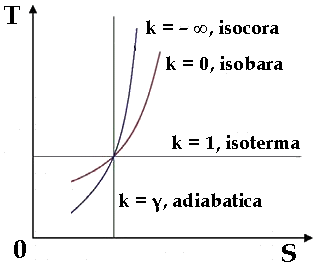
\includegraphics[width=0.5\linewidth]{media/politropiche.png}
    \caption{Principali politropiche sul piano T-S}
\end{figure}

\subsection{Rendimento del ciclo di Carnot}
\label{subsec:rendimento_carnot}
Il rendimento del ciclo di Carnot è definito dalla seguente:
\begin{equation}
    \eta_c \stackrel{def}{=} 1 - \frac{T_{min}}{T_{max}}
\end{equation}
Si definiscono inoltre le temperature medie di adduzione o sottrazione del calore con
\begin{equation}
    T_{\text{media}} \stackrel{def}{=} \left|\frac{q}{\Delta s}\right|
\end{equation}

\section{Bilanci di energia}
\label{sec:bilanci_energia}
Preso un sistema generico è possibile esaminarne le trasformazioni mediante un bilancio
energetico
\begin{equation}
    \label{eq:bilancio_energetico}
    \frac{dE}{dt} = \dot{Q}_c + \dot{Q}_{12} - \dot{L}_{12} + \dot{m}_1
    (p_1v_1 + \frac{c^2_1}{2} + gz_1 + u_1) -p\frac{dV}{dt} - \dot{m}_2
    (p_2v_2 + \frac{c^2_2}{2} + gz_2 + u_2)
\end{equation}

Se il sistema è chiuso la portata massica è nulla, di conseguenza sarà nullo il lavoro
d'elica, quindi la \eqref{eq:bilancio_energetico} diventa:
\begin{equation}
    \label{eq:I_principio_gen_chiusi}
    dQ - pdV = d\left(U+mgz+m\frac{c^2}{2}\right)
\end{equation}

Per sistemi aperti e trasformazioni reversibili, il lavoro di compressione adiabatico
si esprime tramite la seguente:
\begin{equation}
    \label{eq:lavoro_compressione_isoentropico}
    L_{is} = (h_1 - h_2) = - \int_{p_1}^{p_2} v \cdot dp
\end{equation}

Se la trasformazione non è isoentropica, vale la disuguaglianza
\begin{equation}
    L_r = (h_1 - h_2) > - \int_{p_1}^{p_2} v \cdot dp
\end{equation}
ossia l'energia globalmente fornita al fluido è maggiore della variazione di
energia di pressione

Si definisce quindi rendimento di compressione isoentropico il rapporto
\begin{equation}
    \label{eq:rendimento_compressione}
    \eta_c \stackrel{def}{=} \frac{- \displaystyle \int_{p_1}^{p_2} v \cdot dp}{h_1 - h_2} = \frac{L_{is}}{L_r}
    %uso \displaystyle per forzare l'integrale grande
\end{equation}


\end{document}
